% ------------------------------------------------------------------------------
% TYPO3 CMS 6.2 LTS - What's New - Chapter "TypoScript" (Dutch Version)
%
% @author	Christiaan Wiesenekker <cwiesenekker@gmail.com>
% @author	Ric van Westhreenen <ric.vanwesthreenen@typo3.org>
% @license	Creative Commons BY-NC-SA 3.0
% @link		http://typo3.org/download/release-notes/whats-new/
% @language	Dutch
% ------------------------------------------------------------------------------
% Chapter: TypoScript
% ------------------------------------------------------------------------------

\section{TSconfig \& TypoScript}
\begin{frame}[fragile]
	\frametitle{TSconfig \& TypoScript}

	\begin{center}\huge{Hoofdstuk 4:}\end{center}
	\begin{center}\huge{\color{typo3darkgrey}\textbf{TSconfig \& TypoScript}}\end{center}

\end{frame}

% ------------------------------------------------------------------------------
% Include TypoScript
% ------------------------------------------------------------------------------
% http://forge.typo3.org/issues/34621

\begin{frame}[fragile]
	\frametitle{TSconfig \& TypoScript}
	\framesubtitle{Include TypoScript}

	\begin{itemize}
		\item Include alle TypoScript bestanden vanuit een map(recursief)

			\lstinline!<INCLUDE_TYPOSCRIPT: source="DIR:directory">!
			\lstinline!<INCLUDE_TYPOSCRIPT: source="DIR:EXT:myextension/res/setup">!

		\item De volgorde waarni bestanden worden geinclude:\newline
			alfabetisch, dan bestanden, daarna mappen
			\item Limiteer bestanden die worden geinclude door extensies aan te geven\texttt{extensions="..."}

			\lstinline!<INCLUDE_TYPOSCRIPT: source="DIR:directory" extensions="ts">!

		\item Standaard worden alleen de bestanden met de extentie ts, t3, t3s, t3c, txt geinclude
		\item Deze lijst is configureer (Install Tool):\newline
			\texttt{\$TYPO3\_CONF\_VARS['SYS']['tsfile\_ext']}
	\end{itemize}

\end{frame}

% ------------------------------------------------------------------------------
% Include TypoScript
% ------------------------------------------------------------------------------
% http://forge.typo3.org/issues/52018

\begin{frame}[fragile]
	\frametitle{TSconfig \& TypoScript}
	\framesubtitle{Include TypoScript}

	\begin{itemize}
		\item Relatieve paden kunnen worden doorgegeven aan \texttt{INCLUDE\_TYPOSCRIPT},\newline
			als de doorgeving recursief wordt aangevraagd vanaf een bestand
		\item Eerste include \textbf{MOET} absoluut zijn
		\item \texttt{./} toont de actuele map van de laatste include
		\item \texttt{../} toont de bovenliggende map van de laatste include
		\item Voorbeelden:

			\lstinline!<INCLUDE_TYPOSCRIPT: source="FILE:directory/typoscript/setup.ts">!
			\lstinline!<INCLUDE_TYPOSCRIPT: source="FILE:./filename.ts">!
			\lstinline!<INCLUDE_TYPOSCRIPT: source="FILE:../filename.ts">!
			\lstinline!<INCLUDE_TYPOSCRIPT: source="FILE:../directory/filename.ts">!

	\end{itemize}

\end{frame}

% ------------------------------------------------------------------------------
% stdWrap for strPad
% ------------------------------------------------------------------------------
% http://forge.typo3.org/issues/43604

\begin{frame}[fragile]
	\frametitle{TSconfig \& TypoScript}
	\framesubtitle{strPad}

	\begin{itemize}
		\item Optie \texttt{stdWrap} is toegevoegd aan de \texttt{strPad} eigenschappen

			\begin{lstlisting}
				page = PAGE
				page.10 = TEXT
				page.10 {
				  value = Hello World!
				  strPad {
				    length = 5
				    length {
				      current = 1
				      setCurrent.data = TSFE:page|uid
				      setCurrent.wrap = | + 80
				      prioriCalc = 1
				    }
				    padWith = .
				  }
				}
			\end{lstlisting}

	\end{itemize}

\end{frame}

% ------------------------------------------------------------------------------
% stdWrap for _DEFAULT_PI_VARS
% ------------------------------------------------------------------------------
% http://forge.typo3.org/issues/22045
% http://forge.typo3.org/issues/49314

\begin{frame}[fragile]
	\frametitle{TSconfig \& TypoScript}
	\framesubtitle{\_DEFAULT\_PI\_VARS}

	\begin{itemize}
		\item \texttt{stdWrap} is toegevoegd aan \texttt{\_DEFAULT\_PI\_VARS}
		\item \texttt{\_DEFAULT\_PI\_VARS} worden gebruikt om standaard waardes in te stellen voor piVars (GET/POST variables for an extension)

		\item TYPO3 < 6.2
			\begin{lstlisting}
				plugin.tt_news._DEFAULT_PI_VARS {
				  year = 2014
				}
			\end{lstlisting}

		\item TYPO3 >= 6.2
			\begin{lstlisting}
				plugin.tt_news._DEFAULT_PI_VARS {
				  year.stdWrap.data = date:Y
				}
			\end{lstlisting}

	\end{itemize}

\end{frame}

% ------------------------------------------------------------------------------
% Debug Register and Page
% ------------------------------------------------------------------------------
% http://forge.typo3.org/issues/49478

\begin{frame}[fragile]
	\frametitle{TSconfig \& TypoScript}
	\framesubtitle{Debug Output}

	\begin{columns}[T]

		\begin{column}{.6\textwidth}
			\begin{itemize}
				\item De uitkomst voor het register en pagina variabelen:\newline
					\texttt{\$GLOBALS['TSFE']->register}\newline
					\texttt{\$GLOBALS['TSFE']->page}

				\item Voorbeeld:

					\begin{lstlisting}
						10 = LOAD_REGISTER
						10.variable = value
					\end{lstlisting}

					\begin{lstlisting}
						20 = TEXT
						20.data = debug:register
					\end{lstlisting}

					\begin{lstlisting}
						30 = TEXT
						30.data = debug:page
					\end{lstlisting}

			\end{itemize}
		\end{column}

		\begin{column}{.4\textwidth}
			\begin{figure}\vspace*{-0.4cm}
				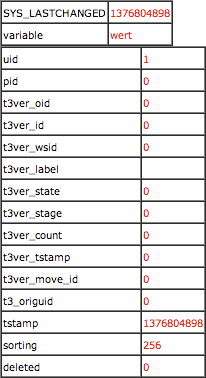
\includegraphics[width=0.6\linewidth]{Images/TypoScript/DebugRegisterAndPage.png}
			\end{figure}
		\end{column}

	\end{columns}

\end{frame}

% ------------------------------------------------------------------------------
% File Links: "register:titleText" and "register:altText"
% ------------------------------------------------------------------------------
% http://forge.typo3.org/issues/44182

\begin{frame}[fragile]
	\frametitle{TSconfig \& TypoScript}
	\framesubtitle{Bestandslinks}

	\begin{itemize}
		\item Bestandslinks bieden een omschrijving, title en een alternatieve titel voor elk bestand. 
			Alle drie kunnen worden benaderd via de registers:

			\begin{itemize}
				\item \texttt{register:description}
				\item \texttt{register:titleText}
				\item \texttt{register:altText}
			\end{itemize}

		\item Voorbeeld:

			\begin{lstlisting}
				# filelinks
				tt_content.uploads.20 {
				  # link description instead of filename
				  labelStdWrap.data = register:description
				  # output alternative text
				  itemRendering.20.data = register:titleText
				}
			\end{lstlisting}

	\end{itemize}

\end{frame}

% ------------------------------------------------------------------------------
% stdWrap replacement: add optionSplit-support
% ------------------------------------------------------------------------------
% http://forge.typo3.org/issues/42287

\begin{frame}[fragile]
	\frametitle{TSconfig \& TypoScript}
	\framesubtitle{stdWrap functie: vervaninging (1)}

	\begin{itemize}
		\item Optie \texttt{replace} van \texttt{stdWrap}-functie \texttt{replacement}\newline
			ondersteund \texttt{optionSplit} nu

		\item Voorbeeld 1:

			\begin{lstlisting}
				10 = TEXT
				10.value = TYPO3_inspires_people_to_share
				10.replacement.10 {
				  search = _
				  replace = 1 || 2 || 3
				  useOptionSplitReplace = 1
				}
			\end{lstlisting}

			Output:\newline
				\texttt{TYPO31inspires2people3to3share}

	\end{itemize}

\end{frame}

% ------------------------------------------------------------------------------
% stdWrap replacement: add optionSplit-support
% ------------------------------------------------------------------------------
% http://forge.typo3.org/issues/42287

\begin{frame}[fragile]
	\frametitle{TSconfig \& TypoScript}
	\framesubtitle{stdWrap functie: vervanging (2)}

	\begin{itemize}
		\item Optie \texttt{replace} of \texttt{stdWrap}-functie \texttt{replacement}\newline
			ondersteund \texttt{optionSplit} nu

		\item Voorbeeld 2:

			\begin{lstlisting}
				10 = TEXT
				10.value = TYPO3 inspires people to share
				10.replacement.10 {
				  search = #(TYPO3|people|share)#i
				  replace = ${1} CMS || all ${1} || collaborate and ${1}
				  useOptionSplitReplace = 1
				  useRegExp = 1
				}
			\end{lstlisting}

			Output:\newline
				\texttt{TYPO3 CMS inspires all people to collaborate and share}

	\end{itemize}

\end{frame}

% ------------------------------------------------------------------------------
% Register values in FilesContentObject
% ------------------------------------------------------------------------------
% http://forge.typo3.org/issues/49480

\begin{frame}[fragile]
	\frametitle{TSconfig \& TypoScript}
	\framesubtitle{cObject FILE}

	\begin{itemize}
		\item Twee registers toegevoegd to cObject FILES:\newline
			\texttt{FILE\_NUM\_CURRENT} and \texttt{FILES\_COUNT}

		\item Voorbeeld:

			\lstset{
				basicstyle=\tiny\ttfamily
			}

			\begin{lstlisting}
				10 = FILES
				10 {
				  references {
				    table = tt_news
				    uid.field = uid
				    fieldName = media
				  }
				  renderObj = COA
				  renderObj {
				    10 = TEXT
				    10.value = Renders first file twice
				    10.if.isFalse.data = register:FILE_NUM_CURRENT
				    20 = TEXT
				    20.value = file {register:FILE_NUM_CURRENT} of {register:FILES_COUNT}
				    20.insertData = 1
				  }
				}
			\end{lstlisting}

	\end{itemize}

\end{frame}

% ------------------------------------------------------------------------------
% Category Menu In TypoScript
% ------------------------------------------------------------------------------
% http://forge.typo3.org/issues/51161

\begin{frame}[fragile]
	\frametitle{TSconfig \& TypoScript}
	\framesubtitle{Categorie Menu}

	\begin{itemize}
		\item Genereer een menu van categorieen in TypoScript

		\item Voorbeeld:

			\lstset{
				basicstyle=\tiny\ttfamily
			}

			\begin{lstlisting}
				page.20 = HMENU
				page.20 {
				  special = categories
				  special {
				    # comma-separated list of categories
				    value = 1
				    # sort by title (stdWrap)
				    sorting = title
				    # sorting "asc" or "desc" (stdWrap)
				    order = desc
				    1 = TMENU
				    1.NO {
				      allWrap = <li> | </li>
				    }
				  }
				}
			\end{lstlisting}

	\end{itemize}

\end{frame}

% ------------------------------------------------------------------------------
% cObject RECORDS with category support
% (slide added in March 2014)
% ------------------------------------------------------------------------------

\begin{frame}[fragile]
	\frametitle{TSconfig \& TypoScript}
	\framesubtitle{Toegang Categorieen}

	\begin{itemize}
		\item eigenschap \texttt{categories} staat toegang toe tot categorieen\newline
			voor de cObject RECORDS

		\item Voorbeeld:

			\lstset{
				basicstyle=\tiny\ttfamily
			}

			\begin{lstlisting}
				# menu of categorized content elements
				categorized_content = RECORDS
				categorized_content {
				  categories.field = selected_categories
				  categories.relation.field = category_field
				  tables = tt_content
				  conf.tt_content = TEXT
				  conf.tt_content {
				    field = header
				    typolink.parameter = {field:pid}#{field:uid}
				    typolink.parameter.insertData = 1
				    wrap = <li>|</li>
				  }
				  wrap = <ul>|</ul>
				}
			\end{lstlisting}

	\end{itemize}

\end{frame}

% ------------------------------------------------------------------------------
% Category Menu In TypoScript
% ------------------------------------------------------------------------------
% http://forge.typo3.org/issues/51782

\begin{frame}[fragile]
	\frametitle{TSconfig \& TypoScript}
	\framesubtitle{CSS en JavaScript bestanden}

	\begin{itemize}
		\item \texttt{splitChar} kan nu worden gedefinieerd voor de \texttt{allWrap} eigenschap 
		\item De wrap werkt nu hetzelfde als de standaard \texttt{stdWrap.wrap} methode 
		\item Standaard \texttt{splitChar}-karakter is het 'pipe' symbool: \texttt{|}
		\item Deze wijzing heeft invloed op:

			\begin{itemize}
				\item \texttt{includeCSS}
				\item \texttt{includeJSlibs}
				\item \texttt{includeJSFooterlibs}
				\item \texttt{includeJS}
				\item \texttt{includeJSFooter}
			\end{itemize}

	\end{itemize}

\end{frame}

% ------------------------------------------------------------------------------
% Conditions: userFunc Accepts Multiple Arguments
% ------------------------------------------------------------------------------
% http://forge.typo3.org/issues/47159

\begin{frame}[fragile]
	\frametitle{TSconfig \& TypoScript}
	\framesubtitle{Condities}

	\begin{itemize}
		\item Conditie \texttt{userFunc} accepteert nu meerdere argumenten 

		\item TYPO3 < 6.2
			\begin{lstlisting}
				[userFunc = user_function(argument1)]
			\end{lstlisting}

		\item TYPO3 >= 6.2
			\begin{lstlisting}
				[userFunc = user_function(argument1, argument2, ...)]
			\end{lstlisting}

		\item Voorbeeld:
			% \texttt{[userFunc = user\_match(checkSubnet, 192.168)]}

			\lstinline![userFunc = user_match(checkSubnet, 192.168)]!

			\begin{lstlisting}
				function user_match($command, $subnet) {
				  switch($command) {
				    case 'checkSubnet':
				      if (strstr(getenv('REMOTE_ADDR'), $subnet)) { ... }
				  }
				}
			\end{lstlisting}

	\end{itemize}

\end{frame}

% ------------------------------------------------------------------------------
% Conditions: Application Context
% ------------------------------------------------------------------------------
% http://forge.typo3.org/issues/39441
% http://forge.typo3.org/issues/50132

\begin{frame}[fragile]
	\frametitle{TSconfig \& TypoScript}
	\framesubtitle{Conditie}

	\begin{itemize}
		\item Applicatie context kan worden bepaald in de condities 
		\item 'Wildcards' "\texttt{+}" en "\texttt{*}" en reguliere expressie worden vanaf nu ondersteund
		\item Voorbeeld:

			\lstset{
				basicstyle=\tiny\ttfamily
			}

			\begin{lstlisting}
				[applicationContext = Development/Debugging, Development/Profiling]
				  # TYPO3 site in development stage
				[global]

				[applicationContext = Production*]
				  # TYPO3 site in production stage
				  # for example "Production/Live" or "Production/Staging"
				[global]

				[applicationContext = /^TestServer\d+$/]
				  # TYPO3 site on TestServer1 or TestServer2 or TestServer3, etc.
				[global]
			\end{lstlisting}

	\end{itemize}

\end{frame}

% ------------------------------------------------------------------------------
% Conditions: IP Supports Keyword devIP
% ------------------------------------------------------------------------------
% http://forge.typo3.org/issues/50092

\begin{frame}[fragile]
	\frametitle{TSconfig \& TypoScript}
	\framesubtitle{Conditie}

	\begin{itemize}

		\item Wanneer je gebruikt maakt van een IP conditie, sleutelwoord \texttt{devIP} kan worden gebruikt om te controelren op het IP adres van de client overeenkomt met de\texttt{devIpMask} instelling in de Installatie Tool
		\item Voorbeeld:

%			\lstset{
%				basicstyle=\tiny\ttfamily
%			}

			\begin{lstlisting}
				[IP = devIP]
				  page.10 = TEXT
				  page.10.value = Hello Developer!
				[global]
			\end{lstlisting}

	\end{itemize}

\end{frame}

% ------------------------------------------------------------------------------
% Records Without Default Translation
% ------------------------------------------------------------------------------
% http://forge.typo3.org/issues/24005

\begin{frame}[fragile]
	\frametitle{TSconfig \& TypoScript}
	\framesubtitle{Records zonder standaard vertaling }

	\begin{itemize}

		\item Nieuwe optie \texttt{includeRecordsWithoutDefaultTranslation}
			verkrijgt records zonder een 'localization parent'\newline
			(maar met het veld \texttt{languageField} die overeenkomt met de huidige taal)

		\item Voorbeeld:

			\begin{lstlisting}
				pageContent = CONTENT
				pageContent {
				  table = tt_content
				  select.includeRecordsWithoutDefaultTranslation = 1
				  ...
				}
			\end{lstlisting}

	\end{itemize}

\end{frame}

% ------------------------------------------------------------------------------
% cObject FILES: begin/maxItems options
% ------------------------------------------------------------------------------
% http://forge.typo3.org/issues/52632

\begin{frame}[fragile]
	\frametitle{TSconfig \& TypoScript}
	\framesubtitle{cObject FILES}

	\begin{itemize}

		\item cObject FILES ondersteund nu \texttt{begin} en \texttt{maxItems} als eigenschappen 

		\item Voorbeeld:

			\lstset{
				basicstyle=\tiny\ttfamily
			}

			\begin{lstlisting}
				page.10 = FILES
				page.10 {
				  references {
				    table = pages
				    uid.data = page:uid
				    fieldName = media
				  }

				  # retrieve up to 5 files, beginning at the first (0):
				  begin = 0
				  maxItems = 5

				  renderObj = TEXT
				  renderObj {
				    data = file:current:size
				    wrap = <p>File size:<strong>|</strong></p>
				  }
				}
			\end{lstlisting}

	\end{itemize}

\end{frame}

% ------------------------------------------------------------------------------
% Exclude doktypes From Pagetree
% ------------------------------------------------------------------------------
% http://forge.typo3.org/issues/49279
% http://forge.typo3.org/issues/49356

\begin{frame}[fragile]
	\frametitle{TSconfig \& TypoScript}
	\framesubtitle{Uitsluiten van doktypes van de Paginaboom}

	\begin{itemize}

		\item Specifieke doktypes kunnen worden uitgesloten van de paginaboom
		\item De configuratie wordt gedaan in UserTSconfig (daardoor is het gebruiker of groep specifiek)
		\item Voorbeeld:

			\begin{lstlisting}
				# exclude "folder" pages
				options.pageTree.excludeDoktypes = 254

				# exclude "folder" and "standard" pages
				options.pageTree.excludeDoktypes = 254,1
			\end{lstlisting}

	\end{itemize}

\end{frame}

% ------------------------------------------------------------------------------
% Hide Modules In Backend
% ------------------------------------------------------------------------------

\begin{frame}[fragile]
	\frametitle{TSconfig \& TypoScript}
	\framesubtitle{Verberg Modules In Backend}

	\begin{itemize}

		\item Modules kunnen worden verborgen in de backend
		\item Dit heeft geen impact op de toegang tot de module\newline
			(gebruikt de ACL voor BE gebruikers en groepen om de beperkingen in te stellen)
		\item Voorbeeld:

			\lstinline!options.hideModules = file, help!
			\lstinline!options.hideModules.web := addToList(func,info)!
			\lstinline!options.hideModules.system = BelogLog!

	\end{itemize}

\end{frame}

% ------------------------------------------------------------------------------
% Alternative Domain For Preview
% ------------------------------------------------------------------------------
% http://forge.typo3.org/issues/30889

\begin{frame}[fragile]
	\frametitle{TSconfig \& TypoScript}
	\framesubtitle{Voorbeeld domein}

	\begin{itemize}

		\item Een alternatief domein kan worden ingesteld voor de pagina/site previews in pageTS
		\item Handig wanneer je gebruikt maakt van multidomein websites
		\item Voorbeeld:

			\lstinline!TCEMAIN.viewDomain = example.com!

	\end{itemize}

\end{frame}

% ------------------------------------------------------------------------------
% Conditions in Backend Layouts
% ------------------------------------------------------------------------------
% http://forge.typo3.org/issues/47588

\begin{frame}[fragile]
	\frametitle{TSconfig \& TypoScript}
	\framesubtitle{Condities in  de Backend Layouts}

	\begin{itemize}

		\item Backend layouts ondersteunen nu condities
		\item Voorbeeld:

			\lstset{
				basicstyle=\tiny\ttfamily
			}

			\begin{lstlisting}
				backend_layout {
				  colCount = 2
				  rowCount = 1
				  rows {
				    1 {
				      columns {
				        1.name = Main
				        1.colPos = 0
				        2.name = Right
				        2.colPos = 1
				      }
				    }
				  }
				}

				[PIDupinRootline = 123]
				  # verwijderd de rechterkolom in de tak van pagina ID 123
				  backend_layout.rows.1.columns.2 >
				[global]
			\end{lstlisting}

	\end{itemize}

\end{frame}


% ------------------------------------------------------------------------------
% Miscellaneous
% ------------------------------------------------------------------------------
% http://forge.typo3.org/issues/34597 (showForgotPassword)
% http://forge.typo3.org/issues/50138 (showForgotPassword)
%
% http://forge.typo3.org/issues/19732 (Content-Length)
%
% http://forge.typo3.org/issues/16386 (Indexed Search) - wow: submitted 7 years ago :-)

\begin{frame}[fragile]
	\frametitle{TSconfig \& TypoScript}
	\framesubtitle{Diversen}

	\begin{itemize}

		\item Zet de "Wachtwoord vergeten" link aan of uit met optie \small\texttt{showForgotPassword}\normalsize\newline
			(handig als er meerdere loginforms zijn geinclude door de EXT:felogin extentie op 1 pagina)

		\item HTTP response voegt nu de header \texttt{Content-length} standaard toe

			\begin{itemize}
				\item Zorgt voor meer snelheid bij het renderen wanneer 'pipelining' aanstaat in apache				\item Can be configured by \texttt{config.enableContentLengthHeader}
			\end{itemize}

		\item Resultaten lijst van EXT:indexed\_search heeft nu \texttt{stdWrap}-eigenschappen\newline
			(optie: \texttt{plugin.tx\_indexedsearch.resultlist\_stdWrap})

	\end{itemize}

\end{frame}

% ------------------------------------------------------------------------------

